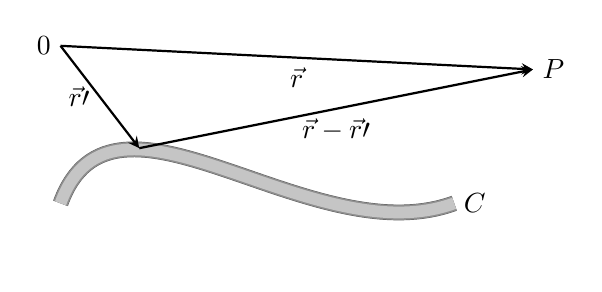
\begin{tikzpicture}
	{   \colorlet{InColor}{gray!25}
		\colorlet{OutColor}{black!75}
		\foreach \I in {1,...,3}
			{   \pgfmathsetlengthmacro{\h}{(\I-1)/3*2mm}
				\pgfmathsetlengthmacro{\r}{sqrt(pow(2mm,2)-pow(\h,2))}
				\pgfmathsetmacro{\c}{(\I-0.5)/3*100}
				\draw[InColor!\c!OutColor, line width=\r] (0,2) to[out=70,in=200] (5,2);
			}
	}
	\draw (5,2) node[right]{$C$};
	\draw (0,4) node[left]{$0$};
	\draw (6,3.7) node[right]{$P$};
	\draw[-stealth,thick] (0,4) -- (1,2.7) node[midway,left]{$\vec{r}\prime $};
	\draw[-stealth,thick] (0,4) -- (6,3.7) node[midway,below]{$\vec{r} $};
	\draw[-stealth,thick] (1,2.7) -- (6,3.7) node[midway,below]{$\vec{r} -\vec{r}\prime $};
\end{tikzpicture}